\documentclass[1p]{elsarticle_modified}
%\bibliographystyle{elsarticle-num}

%\usepackage[colorlinks]{hyperref}
%\usepackage{abbrmath_seonhwa} %\Abb, \Ascr, \Acal ,\Abf, \Afrak
\usepackage{amsfonts}
\usepackage{amssymb}
\usepackage{amsmath}
\usepackage{amsthm}
\usepackage{scalefnt}
\usepackage{amsbsy}
\usepackage{kotex}
\usepackage{caption}
\usepackage{subfig}
\usepackage{color}
\usepackage{graphicx}
\usepackage{xcolor} %% white, black, red, green, blue, cyan, magenta, yellow
\usepackage{float}
\usepackage{setspace}
\usepackage{hyperref}

\usepackage{tikz}
\usetikzlibrary{arrows}

\usepackage{multirow}
\usepackage{array} % fixed length table
\usepackage{hhline}

%%%%%%%%%%%%%%%%%%%%%
\makeatletter
\renewcommand*\env@matrix[1][\arraystretch]{%
	\edef\arraystretch{#1}%
	\hskip -\arraycolsep
	\let\@ifnextchar\new@ifnextchar
	\array{*\c@MaxMatrixCols c}}
\makeatother %https://tex.stackexchange.com/questions/14071/how-can-i-increase-the-line-spacing-in-a-matrix
%%%%%%%%%%%%%%%

\usepackage[normalem]{ulem}

\newcommand{\msout}[1]{\ifmmode\text{\sout{\ensuremath{#1}}}\else\sout{#1}\fi}
%SOURCE: \msout is \stkout macro in https://tex.stackexchange.com/questions/20609/strikeout-in-math-mode

\newcommand{\cancel}[1]{
	\ifmmode
	{\color{red}\msout{#1}}
	\else
	{\color{red}\sout{#1}}
	\fi
}

\newcommand{\add}[1]{
	{\color{blue}\uwave{#1}}
}

\newcommand{\replace}[2]{
	\ifmmode
	{\color{red}\msout{#1}}{\color{blue}\uwave{#2}}
	\else
	{\color{red}\sout{#1}}{\color{blue}\uwave{#2}}
	\fi
}

\newcommand{\Sol}{\mathcal{S}} %segment
\newcommand{\D}{D} %diagram
\newcommand{\A}{\mathcal{A}} %arc


%%%%%%%%%%%%%%%%%%%%%%%%%%%%%5 test

\def\sl{\operatorname{\textup{SL}}(2,\Cbb)}
\def\psl{\operatorname{\textup{PSL}}(2,\Cbb)}
\def\quan{\mkern 1mu \triangleright \mkern 1mu}

\theoremstyle{definition}
\newtheorem{thm}{Theorem}[section]
\newtheorem{prop}[thm]{Proposition}
\newtheorem{lem}[thm]{Lemma}
\newtheorem{ques}[thm]{Question}
\newtheorem{cor}[thm]{Corollary}
\newtheorem{defn}[thm]{Definition}
\newtheorem{exam}[thm]{Example}
\newtheorem{rmk}[thm]{Remark}
\newtheorem{alg}[thm]{Algorithm}

\newcommand{\I}{\sqrt{-1}}
\begin{document}

%\begin{frontmatter}
%
%\title{Boundary parabolic representations of knots up to 8 crossings}
%
%%% Group authors per affiliation:
%\author{Yunhi Cho} 
%\address{Department of Mathematics, University of Seoul, Seoul, Korea}
%\ead{yhcho@uos.ac.kr}
%
%
%\author{Seonhwa Kim} %\fnref{s_kim}}
%\address{Center for Geometry and Physics, Institute for Basic Science, Pohang, 37673, Korea}
%\ead{ryeona17@ibs.re.kr}
%
%\author{Hyuk Kim}
%\address{Department of Mathematical Sciences, Seoul National University, Seoul 08826, Korea}
%\ead{hyukkim@snu.ac.kr}
%
%\author{Seokbeom Yoon}
%\address{Department of Mathematical Sciences, Seoul National University, Seoul, 08826,  Korea}
%\ead{sbyoon15@snu.ac.kr}
%
%\begin{abstract}
%We find all boundary parabolic representation of knots up to 8 crossings.
%
%\end{abstract}
%\begin{keyword}
%    \MSC[2010] 57M25 
%\end{keyword}
%
%\end{frontmatter}

%\linenumbers
%\tableofcontents
%
\newcommand\colored[1]{\textcolor{white}{\rule[-0.35ex]{0.8em}{1.4ex}}\kern-0.8em\color{red} #1}%
%\newcommand\colored[1]{\textcolor{white}{ #1}\kern-2.17ex	\textcolor{white}{ #1}\kern-1.81ex	\textcolor{white}{ #1}\kern-2.15ex\color{red}#1	}

{\Large $\underline{12a_{0995}~(K12a_{0995})}$}

\setlength{\tabcolsep}{10pt}
\renewcommand{\arraystretch}{1.6}
\vspace{1cm}\begin{tabular}{m{100pt}>{\centering\arraybackslash}m{274pt}}
\multirow{5}{120pt}{
	\centering
	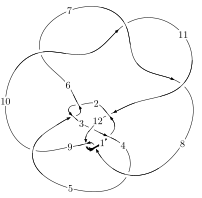
\includegraphics[width=112pt]{../../../GIT/diagram.site/Diagrams/png/1796_12a_0995.png}\\
\ \ \ A knot diagram\footnotemark}&
\allowdisplaybreaks
\textbf{Linearized knot diagam} \\
\cline{2-2}
 &
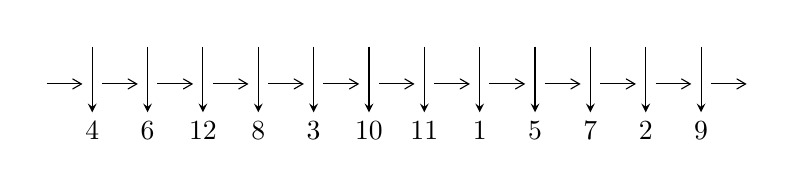
\begin{tikzpicture}[x=20pt, y=17pt]
	% nodes
	\node (C0) at (0, 0) {};
	\node (C1) at (1, 0) {};
	\node (C1U) at (1, +1) {};
	\node (C1D) at (1, -1) {4};

	\node (C2) at (2, 0) {};
	\node (C2U) at (2, +1) {};
	\node (C2D) at (2, -1) {6};

	\node (C3) at (3, 0) {};
	\node (C3U) at (3, +1) {};
	\node (C3D) at (3, -1) {12};

	\node (C4) at (4, 0) {};
	\node (C4U) at (4, +1) {};
	\node (C4D) at (4, -1) {8};

	\node (C5) at (5, 0) {};
	\node (C5U) at (5, +1) {};
	\node (C5D) at (5, -1) {3};

	\node (C6) at (6, 0) {};
	\node (C6U) at (6, +1) {};
	\node (C6D) at (6, -1) {10};

	\node (C7) at (7, 0) {};
	\node (C7U) at (7, +1) {};
	\node (C7D) at (7, -1) {11};

	\node (C8) at (8, 0) {};
	\node (C8U) at (8, +1) {};
	\node (C8D) at (8, -1) {1};

	\node (C9) at (9, 0) {};
	\node (C9U) at (9, +1) {};
	\node (C9D) at (9, -1) {5};

	\node (C10) at (10, 0) {};
	\node (C10U) at (10, +1) {};
	\node (C10D) at (10, -1) {7};

	\node (C11) at (11, 0) {};
	\node (C11U) at (11, +1) {};
	\node (C11D) at (11, -1) {2};

	\node (C12) at (12, 0) {};
	\node (C12U) at (12, +1) {};
	\node (C12D) at (12, -1) {9};
	\node (C13) at (13, 0) {};

	% arrows
	\draw[->,>={angle 60}]
	(C0) edge (C1) (C1) edge (C2) (C2) edge (C3) (C3) edge (C4) (C4) edge (C5) (C5) edge (C6) (C6) edge (C7) (C7) edge (C8) (C8) edge (C9) (C9) edge (C10) (C10) edge (C11) (C11) edge (C12) (C12) edge (C13) ;	\draw[->,>=stealth]
	(C1U) edge (C1D) (C2U) edge (C2D) (C3U) edge (C3D) (C4U) edge (C4D) (C5U) edge (C5D) (C6U) edge (C6D) (C7U) edge (C7D) (C8U) edge (C8D) (C9U) edge (C9D) (C10U) edge (C10D) (C11U) edge (C11D) (C12U) edge (C12D) ;
	\end{tikzpicture} \\
\hhline{~~} \\& 
\textbf{Solving Sequence} \\ \cline{2-2} 
 &
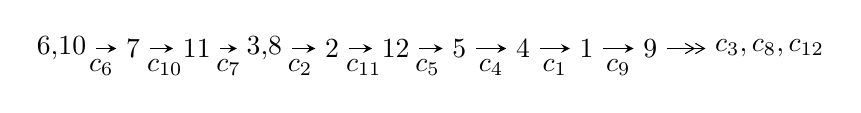
\begin{tikzpicture}[x=23pt, y=7pt]
	% node
	\node (A0) at (-1/8, 0) {6,10};
	\node (A1) at (1, 0) {7};
	\node (A2) at (2, 0) {11};
	\node (A3) at (49/16, 0) {3,8};
	\node (A4) at (33/8, 0) {2};
	\node (A5) at (41/8, 0) {12};
	\node (A6) at (49/8, 0) {5};
	\node (A7) at (57/8, 0) {4};
	\node (A8) at (65/8, 0) {1};
	\node (A9) at (73/8, 0) {9};
	\node (C1) at (1/2, -1) {$c_{6}$};
	\node (C2) at (3/2, -1) {$c_{10}$};
	\node (C3) at (5/2, -1) {$c_{7}$};
	\node (C4) at (29/8, -1) {$c_{2}$};
	\node (C5) at (37/8, -1) {$c_{11}$};
	\node (C6) at (45/8, -1) {$c_{5}$};
	\node (C7) at (53/8, -1) {$c_{4}$};
	\node (C8) at (61/8, -1) {$c_{1}$};
	\node (C9) at (69/8, -1) {$c_{9}$};
	\node (A10) at (11, 0) {$c_{3},c_{8},c_{12}$};

	% edge
	\draw[->,>=stealth]	
	(A0) edge (A1) (A1) edge (A2) (A2) edge (A3) (A3) edge (A4) (A4) edge (A5) (A5) edge (A6) (A6) edge (A7) (A7) edge (A8) (A8) edge (A9) ;
	\draw[->>,>={angle 60}]	
	(A9) edge (A10);
\end{tikzpicture} \\ 

\end{tabular} \\

\footnotetext{
The image of knot diagram is generated by the software ``\textbf{Draw programme}" developed by Andrew Bartholomew(\url{http://www.layer8.co.uk/maths/draw/index.htm\#Running-draw}), where we modified some parts for our purpose(\url{https://github.com/CATsTAILs/LinksPainter}).
}\phantom \\ \newline 
\centering \textbf{Ideals for irreducible components\footnotemark of $X_{\text{par}}$} 
 
\begin{align*}
I^u_{1}&=\langle 
-3.35632\times10^{467} u^{150}-8.69041\times10^{467} u^{149}+\cdots+6.73414\times10^{467} b+6.93806\times10^{467},\\
\phantom{I^u_{1}}&\phantom{= \langle  }2.65827\times10^{466} u^{150}+7.46190\times10^{466} u^{149}+\cdots+3.54428\times10^{466} a-1.15630\times10^{467},\\
\phantom{I^u_{1}}&\phantom{= \langle  }u^{151}+4 u^{150}+\cdots+26 u+1\rangle \\
I^u_{2}&=\langle 
-14417596468648 u^{37}-25796321181488 u^{36}+\cdots+382195085957 b+10825424312466,\\
\phantom{I^u_{2}}&\phantom{= \langle  }14395899214974 u^{37}+25420670905160 u^{36}+\cdots+382195085957 a-10347718637805,\\
\phantom{I^u_{2}}&\phantom{= \langle  }u^{38}+3 u^{37}+\cdots- u-1\rangle \\
\\
\end{align*}
\raggedright * 2 irreducible components of $\dim_{\mathbb{C}}=0$, with total 189 representations.\\
\footnotetext{All coefficients of polynomials are rational numbers. But the coefficients are sometimes approximated in decimal forms when there is not enough margin.}
\newpage
\renewcommand{\arraystretch}{1}
\centering \section*{I. $I^u_{1}= \langle -3.36\times10^{467} u^{150}-8.69\times10^{467} u^{149}+\cdots+6.73\times10^{467} b+6.94\times10^{467},\;2.66\times10^{466} u^{150}+7.46\times10^{466} u^{149}+\cdots+3.54\times10^{466} a-1.16\times10^{467},\;u^{151}+4 u^{150}+\cdots+26 u+1 \rangle$}
\flushleft \textbf{(i) Arc colorings}\\
\begin{tabular}{m{7pt} m{180pt} m{7pt} m{180pt} }
\flushright $a_{6}=$&$\begin{pmatrix}1\\0\end{pmatrix}$ \\
\flushright $a_{10}=$&$\begin{pmatrix}0\\u\end{pmatrix}$ \\
\flushright $a_{7}=$&$\begin{pmatrix}1\\u^2\end{pmatrix}$ \\
\flushright $a_{11}=$&$\begin{pmatrix}- u\\- u^3+u\end{pmatrix}$ \\
\flushright $a_{3}=$&$\begin{pmatrix}-0.750016 u^{150}-2.10533 u^{149}+\cdots-84.6390 u+3.26243\\0.498403 u^{150}+1.29050 u^{149}+\cdots+4.04650 u-1.03028\end{pmatrix}$ \\
\flushright $a_{8}=$&$\begin{pmatrix}- u^2+1\\- u^4+2 u^2\end{pmatrix}$ \\
\flushright $a_{2}=$&$\begin{pmatrix}-0.251613 u^{150}-0.814833 u^{149}+\cdots-80.5925 u+2.23215\\0.498403 u^{150}+1.29050 u^{149}+\cdots+4.04650 u-1.03028\end{pmatrix}$ \\
\flushright $a_{12}=$&$\begin{pmatrix}-1.81156 u^{150}-5.12541 u^{149}+\cdots-73.5438 u-3.48296\\0.701601 u^{150}+1.98724 u^{149}+\cdots+17.9096 u+0.546640\end{pmatrix}$ \\
\flushright $a_{5}=$&$\begin{pmatrix}0.762762 u^{150}+2.12787 u^{149}+\cdots-20.7718 u+8.68380\\0.119785 u^{150}+0.277047 u^{149}+\cdots-14.1821 u-1.93078\end{pmatrix}$ \\
\flushright $a_{4}=$&$\begin{pmatrix}1.16708 u^{150}+3.11306 u^{149}+\cdots-25.2460 u+7.13811\\-0.105342 u^{150}-0.345664 u^{149}+\cdots-17.9438 u-2.08478\end{pmatrix}$ \\
\flushright $a_{1}=$&$\begin{pmatrix}-0.917232 u^{150}-2.79859 u^{149}+\cdots-107.834 u-9.34102\\0.486123 u^{150}+1.36162 u^{149}+\cdots+30.0144 u+1.47747\end{pmatrix}$ \\
\flushright $a_{9}=$&$\begin{pmatrix}1.34444 u^{150}+4.03153 u^{149}+\cdots+142.105 u+3.18649\\-0.505240 u^{150}-1.32977 u^{149}+\cdots-21.2376 u-0.205060\end{pmatrix}$\\&\end{tabular}
\flushleft \textbf{(ii) Obstruction class $= -1$}\\~\\
\flushleft \textbf{(iii) Cusp Shapes $= -1.07674 u^{150}-1.80766 u^{149}+\cdots+217.448 u-18.3877$}\\~\\
\newpage\renewcommand{\arraystretch}{1}
\flushleft \textbf{(iv) u-Polynomials at the component}\newline \\
\begin{tabular}{m{50pt}|m{274pt}}
Crossings & \hspace{64pt}u-Polynomials at each crossing \\
\hline $$\begin{aligned}c_{1}\end{aligned}$$&$\begin{aligned}
&u^{151}-9 u^{150}+\cdots-6836 u+1689
\end{aligned}$\\
\hline $$\begin{aligned}c_{2},c_{5}\end{aligned}$$&$\begin{aligned}
&u^{151}+9 u^{150}+\cdots-1990 u+1825
\end{aligned}$\\
\hline $$\begin{aligned}c_{3}\end{aligned}$$&$\begin{aligned}
&u^{151}+3 u^{150}+\cdots+1987 u+97
\end{aligned}$\\
\hline $$\begin{aligned}c_{4}\end{aligned}$$&$\begin{aligned}
&u^{151}+6 u^{150}+\cdots-130250 u+29375
\end{aligned}$\\
\hline $$\begin{aligned}c_{6},c_{7},c_{10}\end{aligned}$$&$\begin{aligned}
&u^{151}+4 u^{150}+\cdots+26 u+1
\end{aligned}$\\
\hline $$\begin{aligned}c_{8},c_{12}\end{aligned}$$&$\begin{aligned}
&u^{151}+46 u^{149}+\cdots+886 u+149
\end{aligned}$\\
\hline $$\begin{aligned}c_{9}\end{aligned}$$&$\begin{aligned}
&u^{151}-2 u^{150}+\cdots-4383642 u+726827
\end{aligned}$\\
\hline $$\begin{aligned}c_{11}\end{aligned}$$&$\begin{aligned}
&u^{151}-15 u^{150}+\cdots-31153 u+6533
\end{aligned}$\\
\hline
\end{tabular}\\~\\
\newpage\renewcommand{\arraystretch}{1}
\flushleft \textbf{(v) Riley Polynomials at the component}\newline \\
\begin{tabular}{m{50pt}|m{274pt}}
Crossings & \hspace{64pt}Riley Polynomials at each crossing \\
\hline $$\begin{aligned}c_{1}\end{aligned}$$&$\begin{aligned}
&y^{151}+21 y^{150}+\cdots-147730430 y-2852721
\end{aligned}$\\
\hline $$\begin{aligned}c_{2},c_{5}\end{aligned}$$&$\begin{aligned}
&y^{151}+79 y^{150}+\cdots-91731950 y-3330625
\end{aligned}$\\
\hline $$\begin{aligned}c_{3}\end{aligned}$$&$\begin{aligned}
&y^{151}+33 y^{150}+\cdots+3420489 y-9409
\end{aligned}$\\
\hline $$\begin{aligned}c_{4}\end{aligned}$$&$\begin{aligned}
&y^{151}+8 y^{150}+\cdots-145840000000 y-862890625
\end{aligned}$\\
\hline $$\begin{aligned}c_{6},c_{7},c_{10}\end{aligned}$$&$\begin{aligned}
&y^{151}-146 y^{150}+\cdots+122 y-1
\end{aligned}$\\
\hline $$\begin{aligned}c_{8},c_{12}\end{aligned}$$&$\begin{aligned}
&y^{151}+92 y^{150}+\cdots-812880 y-22201
\end{aligned}$\\
\hline $$\begin{aligned}c_{9}\end{aligned}$$&$\begin{aligned}
&y^{151}+2 y^{150}+\cdots+63007761680138 y-528277487929
\end{aligned}$\\
\hline $$\begin{aligned}c_{11}\end{aligned}$$&$\begin{aligned}
&y^{151}-15 y^{150}+\cdots-3528388777 y-42680089
\end{aligned}$\\
\hline
\end{tabular}\\~\\
\newpage\flushleft \textbf{(vi) Complex Volumes and Cusp Shapes}
$$\begin{array}{c|c|c}  
\text{Solutions to }I^u_{1}& \I (\text{vol} + \sqrt{-1}CS) & \text{Cusp shape}\\
 \hline 
\begin{aligned}
u &= -0.395913 + 0.922675 I \\
a &= \phantom{-}0.30920 + 1.74932 I \\
b &= \phantom{-}0.539768 - 1.161120 I\end{aligned}
 & \phantom{-}1.82224 + 8.97850 I & \phantom{-0.000000 } 0 \\ \hline\begin{aligned}
u &= -0.395913 - 0.922675 I \\
a &= \phantom{-}0.30920 - 1.74932 I \\
b &= \phantom{-}0.539768 + 1.161120 I\end{aligned}
 & \phantom{-}1.82224 - 8.97850 I & \phantom{-0.000000 } 0 \\ \hline\begin{aligned}
u &= \phantom{-}0.432562 + 0.907676 I \\
a &= \phantom{-}0.58466 - 1.72016 I \\
b &= \phantom{-}0.329417 + 1.132480 I\end{aligned}
 & \phantom{-}7.43003 - 3.11821 I & \phantom{-0.000000 } 0 \\ \hline\begin{aligned}
u &= \phantom{-}0.432562 - 0.907676 I \\
a &= \phantom{-}0.58466 + 1.72016 I \\
b &= \phantom{-}0.329417 - 1.132480 I\end{aligned}
 & \phantom{-}7.43003 + 3.11821 I & \phantom{-0.000000 } 0 \\ \hline\begin{aligned}
u &= \phantom{-}0.398506 + 0.910380 I \\
a &= \phantom{-}0.25475 - 1.88780 I \\
b &= \phantom{-}0.581934 + 1.258300 I\end{aligned}
 & \phantom{-}5.7689 - 15.1043 I & \phantom{-0.000000 } 0 \\ \hline\begin{aligned}
u &= \phantom{-}0.398506 - 0.910380 I \\
a &= \phantom{-}0.25475 + 1.88780 I \\
b &= \phantom{-}0.581934 - 1.258300 I\end{aligned}
 & \phantom{-}5.7689 + 15.1043 I & \phantom{-0.000000 } 0 \\ \hline\begin{aligned}
u &= \phantom{-}1.051460 + 0.031799 I \\
a &= \phantom{-}0.572699 + 0.846716 I \\
b &= -0.220280 - 1.212270 I\end{aligned}
 & \phantom{-}1.50497 - 3.62679 I & \phantom{-0.000000 } 0 \\ \hline\begin{aligned}
u &= \phantom{-}1.051460 - 0.031799 I \\
a &= \phantom{-}0.572699 - 0.846716 I \\
b &= -0.220280 + 1.212270 I\end{aligned}
 & \phantom{-}1.50497 + 3.62679 I & \phantom{-0.000000 } 0 \\ \hline\begin{aligned}
u &= -0.598347 + 0.666097 I \\
a &= -0.16850 - 1.52968 I \\
b &= -0.478723 + 1.274520 I\end{aligned}
 & \phantom{-}3.59961 + 5.85301 I & \phantom{-0.000000 } 0 \\ \hline\begin{aligned}
u &= -0.598347 - 0.666097 I \\
a &= -0.16850 + 1.52968 I \\
b &= -0.478723 - 1.274520 I\end{aligned}
 & \phantom{-}3.59961 - 5.85301 I & \phantom{-0.000000 } 0\\
 \hline 
 \end{array}$$\newpage$$\begin{array}{c|c|c}  
\text{Solutions to }I^u_{1}& \I (\text{vol} + \sqrt{-1}CS) & \text{Cusp shape}\\
 \hline 
\begin{aligned}
u &= -0.790166 + 0.419125 I \\
a &= \phantom{-}0.923399 + 0.679091 I \\
b &= -0.172002 - 0.888623 I\end{aligned}
 & -0.026731 + 0.249329 I & \phantom{-0.000000 } 0 \\ \hline\begin{aligned}
u &= -0.790166 - 0.419125 I \\
a &= \phantom{-}0.923399 - 0.679091 I \\
b &= -0.172002 + 0.888623 I\end{aligned}
 & -0.026731 - 0.249329 I & \phantom{-0.000000 } 0 \\ \hline\begin{aligned}
u &= \phantom{-}0.862566 + 0.769640 I \\
a &= -0.658978 + 0.892280 I \\
b &= \phantom{-}0.462248 - 1.114990 I\end{aligned}
 & \phantom{-}4.43962 + 9.42483 I & \phantom{-0.000000 } 0 \\ \hline\begin{aligned}
u &= \phantom{-}0.862566 - 0.769640 I \\
a &= -0.658978 - 0.892280 I \\
b &= \phantom{-}0.462248 + 1.114990 I\end{aligned}
 & \phantom{-}4.43962 - 9.42483 I & \phantom{-0.000000 } 0 \\ \hline\begin{aligned}
u &= -0.899348 + 0.752807 I \\
a &= -0.450036 - 0.841376 I \\
b &= \phantom{-}0.409776 + 1.015980 I\end{aligned}
 & \phantom{-}0.38102 - 3.25469 I & \phantom{-0.000000 } 0 \\ \hline\begin{aligned}
u &= -0.899348 - 0.752807 I \\
a &= -0.450036 + 0.841376 I \\
b &= \phantom{-}0.409776 - 1.015980 I\end{aligned}
 & \phantom{-}0.38102 + 3.25469 I & \phantom{-0.000000 } 0 \\ \hline\begin{aligned}
u &= -0.285479 + 0.776322 I \\
a &= \phantom{-}1.33386 + 1.43737 I \\
b &= -0.228862 - 1.046640 I\end{aligned}
 & \phantom{-}4.65161 - 1.17305 I & \phantom{-0.000000 } 0 \\ \hline\begin{aligned}
u &= -0.285479 - 0.776322 I \\
a &= \phantom{-}1.33386 - 1.43737 I \\
b &= -0.228862 + 1.046640 I\end{aligned}
 & \phantom{-}4.65161 + 1.17305 I & \phantom{-0.000000 } 0 \\ \hline\begin{aligned}
u &= \phantom{-}0.466976 + 1.086610 I \\
a &= -0.05581 + 1.53114 I \\
b &= -0.239066 - 1.124310 I\end{aligned}
 & \phantom{-}6.47214 - 4.06326 I & \phantom{-0.000000 } 0 \\ \hline\begin{aligned}
u &= \phantom{-}0.466976 - 1.086610 I \\
a &= -0.05581 - 1.53114 I \\
b &= -0.239066 + 1.124310 I\end{aligned}
 & \phantom{-}6.47214 + 4.06326 I & \phantom{-0.000000 } 0\\
 \hline 
 \end{array}$$\newpage$$\begin{array}{c|c|c}  
\text{Solutions to }I^u_{1}& \I (\text{vol} + \sqrt{-1}CS) & \text{Cusp shape}\\
 \hline 
\begin{aligned}
u &= -0.467316 + 0.645610 I \\
a &= \phantom{-}0.50155 + 1.73448 I \\
b &= \phantom{-}0.265133 - 0.564344 I\end{aligned}
 & -1.121110 + 0.012098 I & \phantom{-0.000000 } 0 \\ \hline\begin{aligned}
u &= -0.467316 - 0.645610 I \\
a &= \phantom{-}0.50155 - 1.73448 I \\
b &= \phantom{-}0.265133 + 0.564344 I\end{aligned}
 & -1.121110 - 0.012098 I & \phantom{-0.000000 } 0 \\ \hline\begin{aligned}
u &= \phantom{-}0.639968 + 0.473480 I \\
a &= -0.079364 - 0.504106 I \\
b &= \phantom{-}0.352919 - 0.419281 I\end{aligned}
 & \phantom{-}2.60382 - 3.71655 I & \phantom{-0.000000 } 0 \\ \hline\begin{aligned}
u &= \phantom{-}0.639968 - 0.473480 I \\
a &= -0.079364 + 0.504106 I \\
b &= \phantom{-}0.352919 + 0.419281 I\end{aligned}
 & \phantom{-}2.60382 + 3.71655 I & \phantom{-0.000000 } 0 \\ \hline\begin{aligned}
u &= -0.287870 + 0.741226 I \\
a &= -0.03917 - 2.02126 I \\
b &= -0.524280 + 1.132570 I\end{aligned}
 & \phantom{-}1.57214 + 3.89522 I & \phantom{-0.000000 } 0 \\ \hline\begin{aligned}
u &= -0.287870 - 0.741226 I \\
a &= -0.03917 + 2.02126 I \\
b &= -0.524280 - 1.132570 I\end{aligned}
 & \phantom{-}1.57214 - 3.89522 I & \phantom{-0.000000 } 0 \\ \hline\begin{aligned}
u &= \phantom{-}1.198490 + 0.176927 I \\
a &= \phantom{-}1.44258 - 0.34480 I \\
b &= \phantom{-}0.836368 + 0.866080 I\end{aligned}
 & \phantom{-}2.44809 - 7.61183 I & \phantom{-0.000000 } 0 \\ \hline\begin{aligned}
u &= \phantom{-}1.198490 - 0.176927 I \\
a &= \phantom{-}1.44258 + 0.34480 I \\
b &= \phantom{-}0.836368 - 0.866080 I\end{aligned}
 & \phantom{-}2.44809 + 7.61183 I & \phantom{-0.000000 } 0 \\ \hline\begin{aligned}
u &= -1.221370 + 0.080433 I \\
a &= \phantom{-}0.42076 + 1.71830 I \\
b &= -0.15014 - 1.44954 I\end{aligned}
 & \phantom{-}4.28980 - 3.56524 I & \phantom{-0.000000 } 0 \\ \hline\begin{aligned}
u &= -1.221370 - 0.080433 I \\
a &= \phantom{-}0.42076 - 1.71830 I \\
b &= -0.15014 + 1.44954 I\end{aligned}
 & \phantom{-}4.28980 + 3.56524 I & \phantom{-0.000000 } 0\\
 \hline 
 \end{array}$$\newpage$$\begin{array}{c|c|c}  
\text{Solutions to }I^u_{1}& \I (\text{vol} + \sqrt{-1}CS) & \text{Cusp shape}\\
 \hline 
\begin{aligned}
u &= \phantom{-}0.392201 + 0.657414 I \\
a &= -0.642889 + 0.199459 I \\
b &= \phantom{-}1.027630 - 0.163312 I\end{aligned}
 & \phantom{-}2.40740 - 9.40150 I & \phantom{-0.000000 } 0 \\ \hline\begin{aligned}
u &= \phantom{-}0.392201 - 0.657414 I \\
a &= -0.642889 - 0.199459 I \\
b &= \phantom{-}1.027630 + 0.163312 I\end{aligned}
 & \phantom{-}2.40740 + 9.40150 I & \phantom{-0.000000 } 0 \\ \hline\begin{aligned}
u &= \phantom{-}1.233800 + 0.082428 I \\
a &= -0.077203 + 0.973153 I \\
b &= -0.06891 - 1.50286 I\end{aligned}
 & \phantom{-}0.69463 - 3.33644 I & \phantom{-0.000000 } 0 \\ \hline\begin{aligned}
u &= \phantom{-}1.233800 - 0.082428 I \\
a &= -0.077203 - 0.973153 I \\
b &= -0.06891 + 1.50286 I\end{aligned}
 & \phantom{-}0.69463 + 3.33644 I & \phantom{-0.000000 } 0 \\ \hline\begin{aligned}
u &= \phantom{-}0.965997 + 0.776238 I \\
a &= -0.313323 + 1.159710 I \\
b &= \phantom{-}0.175814 - 0.995769 I\end{aligned}
 & \phantom{-}6.05310 - 2.71735 I & \phantom{-0.000000 } 0 \\ \hline\begin{aligned}
u &= \phantom{-}0.965997 - 0.776238 I \\
a &= -0.313323 - 1.159710 I \\
b &= \phantom{-}0.175814 + 0.995769 I\end{aligned}
 & \phantom{-}6.05310 + 2.71735 I & \phantom{-0.000000 } 0 \\ \hline\begin{aligned}
u &= -0.394715 + 0.648092 I \\
a &= -0.322974 - 0.363590 I \\
b &= \phantom{-}0.817048 + 0.245952 I\end{aligned}
 & -0.90520 + 3.98675 I & \phantom{-0.000000 } 0 \\ \hline\begin{aligned}
u &= -0.394715 - 0.648092 I \\
a &= -0.322974 + 0.363590 I \\
b &= \phantom{-}0.817048 - 0.245952 I\end{aligned}
 & -0.90520 - 3.98675 I & \phantom{-0.000000 } 0 \\ \hline\begin{aligned}
u &= \phantom{-}0.470426 + 0.590997 I \\
a &= -0.10378 - 1.77112 I \\
b &= \phantom{-}0.528302 + 0.317611 I\end{aligned}
 & \phantom{-}2.06938 + 5.38468 I & \phantom{-0.000000 } 0 \\ \hline\begin{aligned}
u &= \phantom{-}0.470426 - 0.590997 I \\
a &= -0.10378 + 1.77112 I \\
b &= \phantom{-}0.528302 - 0.317611 I\end{aligned}
 & \phantom{-}2.06938 - 5.38468 I & \phantom{-0.000000 } 0\\
 \hline 
 \end{array}$$\newpage$$\begin{array}{c|c|c}  
\text{Solutions to }I^u_{1}& \I (\text{vol} + \sqrt{-1}CS) & \text{Cusp shape}\\
 \hline 
\begin{aligned}
u &= \phantom{-}0.196281 + 0.707481 I \\
a &= \phantom{-}1.12029 - 1.12234 I \\
b &= -0.060722 + 0.802937 I\end{aligned}
 & \phantom{-}3.55125 + 0.41556 I & \phantom{-0.000000 } 0 \\ \hline\begin{aligned}
u &= \phantom{-}0.196281 - 0.707481 I \\
a &= \phantom{-}1.12029 + 1.12234 I \\
b &= -0.060722 - 0.802937 I\end{aligned}
 & \phantom{-}3.55125 - 0.41556 I & \phantom{-0.000000 } 0 \\ \hline\begin{aligned}
u &= -1.227590 + 0.321086 I \\
a &= \phantom{-}0.025930 - 0.485104 I \\
b &= \phantom{-}0.406478 + 1.190100 I\end{aligned}
 & \phantom{-}1.70515 - 0.70564 I & \phantom{-0.000000 } 0 \\ \hline\begin{aligned}
u &= -1.227590 - 0.321086 I \\
a &= \phantom{-}0.025930 + 0.485104 I \\
b &= \phantom{-}0.406478 - 1.190100 I\end{aligned}
 & \phantom{-}1.70515 + 0.70564 I & \phantom{-0.000000 } 0 \\ \hline\begin{aligned}
u &= \phantom{-}1.275920 + 0.022449 I \\
a &= -2.45049 + 0.53181 I \\
b &= -0.123232 - 0.732183 I\end{aligned}
 & \phantom{-}0.56365 + 5.79801 I & \phantom{-0.000000 } 0 \\ \hline\begin{aligned}
u &= \phantom{-}1.275920 - 0.022449 I \\
a &= -2.45049 - 0.53181 I \\
b &= -0.123232 + 0.732183 I\end{aligned}
 & \phantom{-}0.56365 - 5.79801 I & \phantom{-0.000000 } 0 \\ \hline\begin{aligned}
u &= -1.261800 + 0.214920 I \\
a &= \phantom{-}1.192400 + 0.393611 I \\
b &= \phantom{-}0.580363 - 0.909025 I\end{aligned}
 & -0.50677 + 2.23772 I & \phantom{-0.000000 } 0 \\ \hline\begin{aligned}
u &= -1.261800 - 0.214920 I \\
a &= \phantom{-}1.192400 - 0.393611 I \\
b &= \phantom{-}0.580363 + 0.909025 I\end{aligned}
 & -0.50677 - 2.23772 I & \phantom{-0.000000 } 0 \\ \hline\begin{aligned}
u &= \phantom{-}1.271900 + 0.167056 I \\
a &= \phantom{-}1.172710 - 0.182178 I \\
b &= \phantom{-}0.566156 + 1.187640 I\end{aligned}
 & \phantom{-}3.85134 + 1.89307 I & \phantom{-0.000000 } 0 \\ \hline\begin{aligned}
u &= \phantom{-}1.271900 - 0.167056 I \\
a &= \phantom{-}1.172710 + 0.182178 I \\
b &= \phantom{-}0.566156 - 1.187640 I\end{aligned}
 & \phantom{-}3.85134 - 1.89307 I & \phantom{-0.000000 } 0\\
 \hline 
 \end{array}$$\newpage$$\begin{array}{c|c|c}  
\text{Solutions to }I^u_{1}& \I (\text{vol} + \sqrt{-1}CS) & \text{Cusp shape}\\
 \hline 
\begin{aligned}
u &= \phantom{-}0.290725 + 0.650679 I \\
a &= \phantom{-}0.199721 - 0.356884 I \\
b &= \phantom{-}0.530763 + 0.237368 I\end{aligned}
 & \phantom{-}3.78492 - 0.12194 I & \phantom{-0.000000 } 0 \\ \hline\begin{aligned}
u &= \phantom{-}0.290725 - 0.650679 I \\
a &= \phantom{-}0.199721 + 0.356884 I \\
b &= \phantom{-}0.530763 - 0.237368 I\end{aligned}
 & \phantom{-}3.78492 + 0.12194 I & \phantom{-0.000000 } 0 \\ \hline\begin{aligned}
u &= -1.248970 + 0.334674 I \\
a &= -0.75589 - 1.46384 I \\
b &= -0.500992 + 0.693182 I\end{aligned}
 & -3.82438 + 3.34998 I & \phantom{-0.000000 } 0 \\ \hline\begin{aligned}
u &= -1.248970 - 0.334674 I \\
a &= -0.75589 + 1.46384 I \\
b &= -0.500992 - 0.693182 I\end{aligned}
 & -3.82438 - 3.34998 I & \phantom{-0.000000 } 0 \\ \hline\begin{aligned}
u &= \phantom{-}0.068955 + 0.699239 I \\
a &= \phantom{-}0.14091 + 1.70069 I \\
b &= \phantom{-}0.592341 - 1.094560 I\end{aligned}
 & \phantom{-}5.73729 + 4.43088 I & \phantom{-0.000000 } 0 \\ \hline\begin{aligned}
u &= \phantom{-}0.068955 - 0.699239 I \\
a &= \phantom{-}0.14091 - 1.70069 I \\
b &= \phantom{-}0.592341 + 1.094560 I\end{aligned}
 & \phantom{-}5.73729 - 4.43088 I & \phantom{-0.000000 } 0 \\ \hline\begin{aligned}
u &= \phantom{-}0.265498 + 0.646748 I \\
a &= -0.44365 + 2.56882 I \\
b &= -0.55319 - 1.34067 I\end{aligned}
 & \phantom{-}3.19026 - 6.44191 I & -12.0000 + 11.4713 I \\ \hline\begin{aligned}
u &= \phantom{-}0.265498 - 0.646748 I \\
a &= -0.44365 - 2.56882 I \\
b &= -0.55319 + 1.34067 I\end{aligned}
 & \phantom{-}3.19026 + 6.44191 I & -12.0000 - 11.4713 I \\ \hline\begin{aligned}
u &= -0.128914 + 0.686799 I \\
a &= \phantom{-}0.48784 - 1.91211 I \\
b &= -0.631900 + 0.805408 I\end{aligned}
 & \phantom{-}0.86655 + 3.84705 I & -12.0000 - 7.8791 I \\ \hline\begin{aligned}
u &= -0.128914 - 0.686799 I \\
a &= \phantom{-}0.48784 + 1.91211 I \\
b &= -0.631900 - 0.805408 I\end{aligned}
 & \phantom{-}0.86655 - 3.84705 I & -12.0000 + 7.8791 I\\
 \hline 
 \end{array}$$\newpage$$\begin{array}{c|c|c}  
\text{Solutions to }I^u_{1}& \I (\text{vol} + \sqrt{-1}CS) & \text{Cusp shape}\\
 \hline 
\begin{aligned}
u &= -1.296260 + 0.133686 I \\
a &= -0.262178 - 0.741476 I \\
b &= \phantom{-}0.12648 + 1.75568 I\end{aligned}
 & \phantom{-}3.97356 + 6.66748 I & \phantom{-0.000000 } 0 \\ \hline\begin{aligned}
u &= -1.296260 - 0.133686 I \\
a &= -0.262178 + 0.741476 I \\
b &= \phantom{-}0.12648 - 1.75568 I\end{aligned}
 & \phantom{-}3.97356 - 6.66748 I & \phantom{-0.000000 } 0 \\ \hline\begin{aligned}
u &= -1.308940 + 0.014853 I \\
a &= -1.62132 + 0.66875 I \\
b &= -0.490491 - 0.842042 I\end{aligned}
 & -3.89591 + 0.91839 I & \phantom{-0.000000 } 0 \\ \hline\begin{aligned}
u &= -1.308940 - 0.014853 I \\
a &= -1.62132 - 0.66875 I \\
b &= -0.490491 + 0.842042 I\end{aligned}
 & -3.89591 - 0.91839 I & \phantom{-0.000000 } 0 \\ \hline\begin{aligned}
u &= \phantom{-}1.322800 + 0.009344 I \\
a &= -0.848439 + 1.093570 I \\
b &= -0.54209 - 1.32608 I\end{aligned}
 & -1.48603 - 3.84847 I & \phantom{-0.000000 } 0 \\ \hline\begin{aligned}
u &= \phantom{-}1.322800 - 0.009344 I \\
a &= -0.848439 - 1.093570 I \\
b &= -0.54209 + 1.32608 I\end{aligned}
 & -1.48603 + 3.84847 I & \phantom{-0.000000 } 0 \\ \hline\begin{aligned}
u &= \phantom{-}0.459948 + 0.480036 I \\
a &= -0.742762 + 1.117410 I \\
b &= -0.426714 - 1.166170 I\end{aligned}
 & \phantom{-}2.19251 - 3.91255 I & -9.93504 + 2.80464 I \\ \hline\begin{aligned}
u &= \phantom{-}0.459948 - 0.480036 I \\
a &= -0.742762 - 1.117410 I \\
b &= -0.426714 + 1.166170 I\end{aligned}
 & \phantom{-}2.19251 + 3.91255 I & -9.93504 - 2.80464 I \\ \hline\begin{aligned}
u &= \phantom{-}0.107507 + 0.628166 I \\
a &= \phantom{-}0.78778 - 1.64930 I \\
b &= \phantom{-}0.229799 + 1.109420 I\end{aligned}
 & \phantom{-}3.69200 + 0.88634 I & -5.67830 - 1.96706 I \\ \hline\begin{aligned}
u &= \phantom{-}0.107507 - 0.628166 I \\
a &= \phantom{-}0.78778 + 1.64930 I \\
b &= \phantom{-}0.229799 - 1.109420 I\end{aligned}
 & \phantom{-}3.69200 - 0.88634 I & -5.67830 + 1.96706 I\\
 \hline 
 \end{array}$$\newpage$$\begin{array}{c|c|c}  
\text{Solutions to }I^u_{1}& \I (\text{vol} + \sqrt{-1}CS) & \text{Cusp shape}\\
 \hline 
\begin{aligned}
u &= -1.361760 + 0.136901 I \\
a &= -0.564547 - 0.578178 I \\
b &= -1.297910 - 0.250636 I\end{aligned}
 & -6.02457 + 2.64112 I & \phantom{-0.000000 } 0 \\ \hline\begin{aligned}
u &= -1.361760 - 0.136901 I \\
a &= -0.564547 + 0.578178 I \\
b &= -1.297910 + 0.250636 I\end{aligned}
 & -6.02457 - 2.64112 I & \phantom{-0.000000 } 0 \\ \hline\begin{aligned}
u &= -1.353360 + 0.258344 I \\
a &= \phantom{-}1.023270 + 0.363947 I \\
b &= \phantom{-}0.267150 - 0.491798 I\end{aligned}
 & -1.27388 + 3.07615 I & \phantom{-0.000000 } 0 \\ \hline\begin{aligned}
u &= -1.353360 - 0.258344 I \\
a &= \phantom{-}1.023270 - 0.363947 I \\
b &= \phantom{-}0.267150 + 0.491798 I\end{aligned}
 & -1.27388 - 3.07615 I & \phantom{-0.000000 } 0 \\ \hline\begin{aligned}
u &= \phantom{-}1.388200 + 0.141062 I \\
a &= -0.154978 + 0.438599 I \\
b &= -1.36741 + 0.54957 I\end{aligned}
 & -6.20225 - 0.29066 I & \phantom{-0.000000 } 0 \\ \hline\begin{aligned}
u &= \phantom{-}1.388200 - 0.141062 I \\
a &= -0.154978 - 0.438599 I \\
b &= -1.36741 - 0.54957 I\end{aligned}
 & -6.20225 + 0.29066 I & \phantom{-0.000000 } 0 \\ \hline\begin{aligned}
u &= -1.399770 + 0.062318 I \\
a &= -0.497121 + 0.174045 I \\
b &= -1.37614 - 0.61423 I\end{aligned}
 & -5.97812 - 0.65707 I & \phantom{-0.000000 } 0 \\ \hline\begin{aligned}
u &= -1.399770 - 0.062318 I \\
a &= -0.497121 - 0.174045 I \\
b &= -1.37614 + 0.61423 I\end{aligned}
 & -5.97812 + 0.65707 I & \phantom{-0.000000 } 0 \\ \hline\begin{aligned}
u &= -1.388790 + 0.188853 I \\
a &= \phantom{-}0.266866 - 0.041810 I \\
b &= -0.704926 - 0.828542 I\end{aligned}
 & -3.20648 - 1.42275 I & \phantom{-0.000000 } 0 \\ \hline\begin{aligned}
u &= -1.388790 - 0.188853 I \\
a &= \phantom{-}0.266866 + 0.041810 I \\
b &= -0.704926 + 0.828542 I\end{aligned}
 & -3.20648 + 1.42275 I & \phantom{-0.000000 } 0\\
 \hline 
 \end{array}$$\newpage$$\begin{array}{c|c|c}  
\text{Solutions to }I^u_{1}& \I (\text{vol} + \sqrt{-1}CS) & \text{Cusp shape}\\
 \hline 
\begin{aligned}
u &= \phantom{-}1.394520 + 0.159441 I \\
a &= -1.87179 + 0.17410 I \\
b &= -0.291289 - 1.138590 I\end{aligned}
 & \phantom{-}2.34288 - 7.63921 I & \phantom{-0.000000 } 0 \\ \hline\begin{aligned}
u &= \phantom{-}1.394520 - 0.159441 I \\
a &= -1.87179 - 0.17410 I \\
b &= -0.291289 + 1.138590 I\end{aligned}
 & \phantom{-}2.34288 + 7.63921 I & \phantom{-0.000000 } 0 \\ \hline\begin{aligned}
u &= \phantom{-}1.373330 + 0.292896 I \\
a &= \phantom{-}1.290640 - 0.465002 I \\
b &= -0.046045 + 0.785237 I\end{aligned}
 & -0.52152 - 2.68073 I & \phantom{-0.000000 } 0 \\ \hline\begin{aligned}
u &= \phantom{-}1.373330 - 0.292896 I \\
a &= \phantom{-}1.290640 + 0.465002 I \\
b &= -0.046045 - 0.785237 I\end{aligned}
 & -0.52152 + 2.68073 I & \phantom{-0.000000 } 0 \\ \hline\begin{aligned}
u &= \phantom{-}0.983070 + 1.009910 I \\
a &= \phantom{-}0.469754 - 0.962394 I \\
b &= -0.080777 + 0.895256 I\end{aligned}
 & \phantom{-}5.19721 - 3.03779 I & \phantom{-0.000000 } 0 \\ \hline\begin{aligned}
u &= \phantom{-}0.983070 - 1.009910 I \\
a &= \phantom{-}0.469754 + 0.962394 I \\
b &= -0.080777 - 0.895256 I\end{aligned}
 & \phantom{-}5.19721 + 3.03779 I & \phantom{-0.000000 } 0 \\ \hline\begin{aligned}
u &= \phantom{-}1.38600 + 0.30864 I \\
a &= -0.82841 + 1.23836 I \\
b &= -0.756191 - 1.083990 I\end{aligned}
 & -3.97014 - 7.58303 I & \phantom{-0.000000 } 0 \\ \hline\begin{aligned}
u &= \phantom{-}1.38600 - 0.30864 I \\
a &= -0.82841 - 1.23836 I \\
b &= -0.756191 + 1.083990 I\end{aligned}
 & -3.97014 + 7.58303 I & \phantom{-0.000000 } 0 \\ \hline\begin{aligned}
u &= -1.40763 + 0.25231 I \\
a &= -1.26003 - 1.09906 I \\
b &= -0.69981 + 1.40966 I\end{aligned}
 & -2.16246 + 9.72845 I & \phantom{-0.000000 } 0 \\ \hline\begin{aligned}
u &= -1.40763 - 0.25231 I \\
a &= -1.26003 + 1.09906 I \\
b &= -0.69981 - 1.40966 I\end{aligned}
 & -2.16246 - 9.72845 I & \phantom{-0.000000 } 0\\
 \hline 
 \end{array}$$\newpage$$\begin{array}{c|c|c}  
\text{Solutions to }I^u_{1}& \I (\text{vol} + \sqrt{-1}CS) & \text{Cusp shape}\\
 \hline 
\begin{aligned}
u &= -1.42045 + 0.20751 I \\
a &= \phantom{-}0.592511 + 0.128313 I \\
b &= \phantom{-}0.604947 + 0.174650 I\end{aligned}
 & -1.64361 + 3.17831 I & \phantom{-0.000000 } 0 \\ \hline\begin{aligned}
u &= -1.42045 - 0.20751 I \\
a &= \phantom{-}0.592511 - 0.128313 I \\
b &= \phantom{-}0.604947 - 0.174650 I\end{aligned}
 & -1.64361 - 3.17831 I & \phantom{-0.000000 } 0 \\ \hline\begin{aligned}
u &= \phantom{-}1.43607 + 0.09953 I \\
a &= -0.252449 - 0.039186 I \\
b &= -1.366660 + 0.281304 I\end{aligned}
 & -6.63863 - 1.86881 I & \phantom{-0.000000 } 0 \\ \hline\begin{aligned}
u &= \phantom{-}1.43607 - 0.09953 I \\
a &= -0.252449 + 0.039186 I \\
b &= -1.366660 - 0.281304 I\end{aligned}
 & -6.63863 + 1.86881 I & \phantom{-0.000000 } 0 \\ \hline\begin{aligned}
u &= \phantom{-}1.43790 + 0.14720 I \\
a &= -0.1103850 - 0.0066734 I \\
b &= -0.987233 + 0.285377 I\end{aligned}
 & -6.29510 - 1.52422 I & \phantom{-0.000000 } 0 \\ \hline\begin{aligned}
u &= \phantom{-}1.43790 - 0.14720 I \\
a &= -0.1103850 + 0.0066734 I \\
b &= -0.987233 - 0.285377 I\end{aligned}
 & -6.29510 + 1.52422 I & \phantom{-0.000000 } 0 \\ \hline\begin{aligned}
u &= \phantom{-}1.41835 + 0.29295 I \\
a &= -0.89887 + 1.13729 I \\
b &= -0.74061 - 1.22575 I\end{aligned}
 & -3.87520 - 7.64567 I & \phantom{-0.000000 } 0 \\ \hline\begin{aligned}
u &= \phantom{-}1.41835 - 0.29295 I \\
a &= -0.89887 - 1.13729 I \\
b &= -0.74061 + 1.22575 I\end{aligned}
 & -3.87520 + 7.64567 I & \phantom{-0.000000 } 0 \\ \hline\begin{aligned}
u &= -1.44420 + 0.15774 I \\
a &= \phantom{-}1.33023 + 1.62255 I \\
b &= \phantom{-}0.342815 - 1.142610 I\end{aligned}
 & -2.09785 + 8.62195 I & \phantom{-0.000000 } 0 \\ \hline\begin{aligned}
u &= -1.44420 - 0.15774 I \\
a &= \phantom{-}1.33023 - 1.62255 I \\
b &= \phantom{-}0.342815 + 1.142610 I\end{aligned}
 & -2.09785 - 8.62195 I & \phantom{-0.000000 } 0\\
 \hline 
 \end{array}$$\newpage$$\begin{array}{c|c|c}  
\text{Solutions to }I^u_{1}& \I (\text{vol} + \sqrt{-1}CS) & \text{Cusp shape}\\
 \hline 
\begin{aligned}
u &= \phantom{-}0.482641 + 0.225116 I \\
a &= -0.175110 - 0.409993 I \\
b &= -0.370798 - 0.961784 I\end{aligned}
 & \phantom{-}1.81686 - 3.71061 I & -11.64852 + 7.11033 I \\ \hline\begin{aligned}
u &= \phantom{-}0.482641 - 0.225116 I \\
a &= -0.175110 + 0.409993 I \\
b &= -0.370798 + 0.961784 I\end{aligned}
 & \phantom{-}1.81686 + 3.71061 I & -11.64852 - 7.11033 I \\ \hline\begin{aligned}
u &= \phantom{-}1.45667 + 0.24433 I \\
a &= \phantom{-}0.236039 - 0.195747 I \\
b &= \phantom{-}1.092940 - 0.403525 I\end{aligned}
 & -6.86533 - 7.26367 I & \phantom{-0.000000 } 0 \\ \hline\begin{aligned}
u &= \phantom{-}1.45667 - 0.24433 I \\
a &= \phantom{-}0.236039 + 0.195747 I \\
b &= \phantom{-}1.092940 + 0.403525 I\end{aligned}
 & -6.86533 + 7.26367 I & \phantom{-0.000000 } 0 \\ \hline\begin{aligned}
u &= -1.45603 + 0.24861 I \\
a &= \phantom{-}0.173127 + 0.314033 I \\
b &= \phantom{-}1.283430 + 0.314233 I\end{aligned}
 & -3.53837 + 12.72520 I & \phantom{-0.000000 } 0 \\ \hline\begin{aligned}
u &= -1.45603 - 0.24861 I \\
a &= \phantom{-}0.173127 - 0.314033 I \\
b &= \phantom{-}1.283430 - 0.314233 I\end{aligned}
 & -3.53837 - 12.72520 I & \phantom{-0.000000 } 0 \\ \hline\begin{aligned}
u &= -0.028786 + 0.517740 I \\
a &= \phantom{-}0.81457 + 2.29615 I \\
b &= \phantom{-}0.28053 - 1.45206 I\end{aligned}
 & \phantom{-}7.88035 - 4.42352 I & -1.87054 + 3.58395 I \\ \hline\begin{aligned}
u &= -0.028786 - 0.517740 I \\
a &= \phantom{-}0.81457 - 2.29615 I \\
b &= \phantom{-}0.28053 + 1.45206 I\end{aligned}
 & \phantom{-}7.88035 + 4.42352 I & -1.87054 - 3.58395 I \\ \hline\begin{aligned}
u &= \phantom{-}1.47154 + 0.19362 I \\
a &= \phantom{-}0.90147 - 1.13844 I \\
b &= \phantom{-}0.458659 + 0.994130 I\end{aligned}
 & -7.54568 - 2.89339 I & \phantom{-0.000000 } 0 \\ \hline\begin{aligned}
u &= \phantom{-}1.47154 - 0.19362 I \\
a &= \phantom{-}0.90147 + 1.13844 I \\
b &= \phantom{-}0.458659 - 0.994130 I\end{aligned}
 & -7.54568 + 2.89339 I & \phantom{-0.000000 } 0\\
 \hline 
 \end{array}$$\newpage$$\begin{array}{c|c|c}  
\text{Solutions to }I^u_{1}& \I (\text{vol} + \sqrt{-1}CS) & \text{Cusp shape}\\
 \hline 
\begin{aligned}
u &= -1.48248 + 0.14758 I \\
a &= -0.456361 + 0.205470 I \\
b &= -0.644756 + 0.495195 I\end{aligned}
 & -4.54822 + 5.43952 I & \phantom{-0.000000 } 0 \\ \hline\begin{aligned}
u &= -1.48248 - 0.14758 I \\
a &= -0.456361 - 0.205470 I \\
b &= -0.644756 - 0.495195 I\end{aligned}
 & -4.54822 - 5.43952 I & \phantom{-0.000000 } 0 \\ \hline\begin{aligned}
u &= -1.47633 + 0.20618 I \\
a &= -0.848364 - 0.497921 I \\
b &= -0.748457 + 1.145330 I\end{aligned}
 & -4.08967 + 6.59028 I & \phantom{-0.000000 } 0 \\ \hline\begin{aligned}
u &= -1.47633 - 0.20618 I \\
a &= -0.848364 + 0.497921 I \\
b &= -0.748457 - 1.145330 I\end{aligned}
 & -4.08967 - 6.59028 I & \phantom{-0.000000 } 0 \\ \hline\begin{aligned}
u &= -1.48391 + 0.19171 I \\
a &= \phantom{-}0.590773 + 1.031500 I \\
b &= \phantom{-}0.546235 - 0.874362 I\end{aligned}
 & -4.33484 - 2.49145 I & \phantom{-0.000000 } 0 \\ \hline\begin{aligned}
u &= -1.48391 - 0.19171 I \\
a &= \phantom{-}0.590773 - 1.031500 I \\
b &= \phantom{-}0.546235 + 0.874362 I\end{aligned}
 & -4.33484 + 2.49145 I & \phantom{-0.000000 } 0 \\ \hline\begin{aligned}
u &= -0.165706 + 0.450236 I \\
a &= -2.83180 - 2.91509 I \\
b &= -0.162540 + 1.304730 I\end{aligned}
 & \phantom{-}7.40940 + 5.41990 I & \phantom{-}0.43513 - 7.12665 I \\ \hline\begin{aligned}
u &= -0.165706 - 0.450236 I \\
a &= -2.83180 + 2.91509 I \\
b &= -0.162540 - 1.304730 I\end{aligned}
 & \phantom{-}7.40940 - 5.41990 I & \phantom{-}0.43513 + 7.12665 I \\ \hline\begin{aligned}
u &= -0.445265 + 0.142823 I \\
a &= \phantom{-}1.035940 - 0.399197 I \\
b &= -0.885753 - 0.258938 I\end{aligned}
 & -0.87833 - 1.17215 I & -16.9095 + 3.7953 I \\ \hline\begin{aligned}
u &= -0.445265 - 0.142823 I \\
a &= \phantom{-}1.035940 + 0.399197 I \\
b &= -0.885753 + 0.258938 I\end{aligned}
 & -0.87833 + 1.17215 I & -16.9095 - 3.7953 I\\
 \hline 
 \end{array}$$\newpage$$\begin{array}{c|c|c}  
\text{Solutions to }I^u_{1}& \I (\text{vol} + \sqrt{-1}CS) & \text{Cusp shape}\\
 \hline 
\begin{aligned}
u &= -1.49380 + 0.34827 I \\
a &= \phantom{-}1.00962 + 1.09612 I \\
b &= \phantom{-}0.70583 - 1.32097 I\end{aligned}
 & -0.3035 + 19.6529 I & \phantom{-0.000000 } 0 \\ \hline\begin{aligned}
u &= -1.49380 - 0.34827 I \\
a &= \phantom{-}1.00962 - 1.09612 I \\
b &= \phantom{-}0.70583 + 1.32097 I\end{aligned}
 & -0.3035 - 19.6529 I & \phantom{-0.000000 } 0 \\ \hline\begin{aligned}
u &= -0.458680 + 0.077305 I \\
a &= \phantom{-}3.31078 + 1.12935 I \\
b &= \phantom{-}0.097322 - 0.668829 I\end{aligned}
 & -0.687739 + 0.795629 I & -14.2212 - 7.9793 I \\ \hline\begin{aligned}
u &= -0.458680 - 0.077305 I \\
a &= \phantom{-}3.31078 - 1.12935 I \\
b &= \phantom{-}0.097322 + 0.668829 I\end{aligned}
 & -0.687739 - 0.795629 I & -14.2212 + 7.9793 I \\ \hline\begin{aligned}
u &= \phantom{-}1.51374 + 0.25636 I \\
a &= -0.663338 + 0.810282 I \\
b &= -0.77519 - 1.35395 I\end{aligned}
 & -3.19998 - 9.31869 I & \phantom{-0.000000 } 0 \\ \hline\begin{aligned}
u &= \phantom{-}1.51374 - 0.25636 I \\
a &= -0.663338 - 0.810282 I \\
b &= -0.77519 + 1.35395 I\end{aligned}
 & -3.19998 + 9.31869 I & \phantom{-0.000000 } 0 \\ \hline\begin{aligned}
u &= \phantom{-}1.49706 + 0.35112 I \\
a &= \phantom{-}0.99643 - 1.02943 I \\
b &= \phantom{-}0.678137 + 1.220980 I\end{aligned}
 & -4.2594 - 13.5773 I & \phantom{-0.000000 } 0 \\ \hline\begin{aligned}
u &= \phantom{-}1.49706 - 0.35112 I \\
a &= \phantom{-}0.99643 + 1.02943 I \\
b &= \phantom{-}0.678137 - 1.220980 I\end{aligned}
 & -4.2594 + 13.5773 I & \phantom{-0.000000 } 0 \\ \hline\begin{aligned}
u &= -1.51250 + 0.33148 I \\
a &= \phantom{-}1.08247 + 0.93181 I \\
b &= \phantom{-}0.495184 - 1.155070 I\end{aligned}
 & \phantom{-}1.14976 + 7.58504 I & \phantom{-0.000000 } 0 \\ \hline\begin{aligned}
u &= -1.51250 - 0.33148 I \\
a &= \phantom{-}1.08247 - 0.93181 I \\
b &= \phantom{-}0.495184 + 1.155070 I\end{aligned}
 & \phantom{-}1.14976 - 7.58504 I & \phantom{-0.000000 } 0\\
 \hline 
 \end{array}$$\newpage$$\begin{array}{c|c|c}  
\text{Solutions to }I^u_{1}& \I (\text{vol} + \sqrt{-1}CS) & \text{Cusp shape}\\
 \hline 
\begin{aligned}
u &= -1.50399 + 0.39832 I \\
a &= -0.615515 - 1.085130 I \\
b &= -0.446157 + 1.299990 I\end{aligned}
 & \phantom{-}0.26179 + 9.32717 I & \phantom{-0.000000 } 0 \\ \hline\begin{aligned}
u &= -1.50399 - 0.39832 I \\
a &= -0.615515 + 1.085130 I \\
b &= -0.446157 - 1.299990 I\end{aligned}
 & \phantom{-}0.26179 - 9.32717 I & \phantom{-0.000000 } 0 \\ \hline\begin{aligned}
u &= -1.55238 + 0.12872 I \\
a &= \phantom{-}0.028752 + 0.539203 I \\
b &= \phantom{-}0.143653 + 0.350303 I\end{aligned}
 & -4.68327 + 5.84719 I & \phantom{-0.000000 } 0 \\ \hline\begin{aligned}
u &= -1.55238 - 0.12872 I \\
a &= \phantom{-}0.028752 - 0.539203 I \\
b &= \phantom{-}0.143653 - 0.350303 I\end{aligned}
 & -4.68327 - 5.84719 I & \phantom{-0.000000 } 0 \\ \hline\begin{aligned}
u &= \phantom{-}0.293368 + 0.325282 I \\
a &= \phantom{-}2.22644 - 5.15575 I \\
b &= \phantom{-}0.273689 + 0.932741 I\end{aligned}
 & \phantom{-}3.65495 - 6.65848 I & -7.5941 + 13.3955 I \\ \hline\begin{aligned}
u &= \phantom{-}0.293368 - 0.325282 I \\
a &= \phantom{-}2.22644 + 5.15575 I \\
b &= \phantom{-}0.273689 - 0.932741 I\end{aligned}
 & \phantom{-}3.65495 + 6.65848 I & -7.5941 - 13.3955 I \\ \hline\begin{aligned}
u &= \phantom{-}0.299744 + 0.281324 I \\
a &= \phantom{-}2.14422 - 0.94982 I \\
b &= -0.429702 + 1.088460 I\end{aligned}
 & \phantom{-}2.02119 + 3.47303 I & -11.57548 - 3.68608 I \\ \hline\begin{aligned}
u &= \phantom{-}0.299744 - 0.281324 I \\
a &= \phantom{-}2.14422 + 0.94982 I \\
b &= -0.429702 - 1.088460 I\end{aligned}
 & \phantom{-}2.02119 - 3.47303 I & -11.57548 + 3.68608 I \\ \hline\begin{aligned}
u &= \phantom{-}1.60842 + 0.05916 I \\
a &= \phantom{-}0.284118 + 0.039038 I \\
b &= \phantom{-}0.410167 - 0.623452 I\end{aligned}
 & -8.77342 + 0.82140 I & \phantom{-0.000000 } 0 \\ \hline\begin{aligned}
u &= \phantom{-}1.60842 - 0.05916 I \\
a &= \phantom{-}0.284118 - 0.039038 I \\
b &= \phantom{-}0.410167 + 0.623452 I\end{aligned}
 & -8.77342 - 0.82140 I & \phantom{-0.000000 } 0\\
 \hline 
 \end{array}$$\newpage$$\begin{array}{c|c|c}  
\text{Solutions to }I^u_{1}& \I (\text{vol} + \sqrt{-1}CS) & \text{Cusp shape}\\
 \hline 
\begin{aligned}
u &= -0.160233 + 0.351246 I \\
a &= \phantom{-}0.85875 + 1.54908 I \\
b &= -0.449690 - 0.068646 I\end{aligned}
 & -0.697061 - 0.212567 I & -13.66753 + 0.13954 I \\ \hline\begin{aligned}
u &= -0.160233 - 0.351246 I \\
a &= \phantom{-}0.85875 - 1.54908 I \\
b &= -0.449690 + 0.068646 I\end{aligned}
 & -0.697061 + 0.212567 I & -13.66753 - 0.13954 I \\ \hline\begin{aligned}
u &= \phantom{-}0.248350 + 0.280663 I \\
a &= \phantom{-}0.78367 + 1.20017 I \\
b &= -0.970508 - 0.062762 I\end{aligned}
 & -1.09332 - 0.92676 I & -15.5657 + 7.3109 I \\ \hline\begin{aligned}
u &= \phantom{-}0.248350 - 0.280663 I \\
a &= \phantom{-}0.78367 - 1.20017 I \\
b &= -0.970508 + 0.062762 I\end{aligned}
 & -1.09332 + 0.92676 I & -15.5657 - 7.3109 I \\ \hline\begin{aligned}
u &= -0.364852\phantom{ +0.000000I} \\
a &= \phantom{-}1.08276\phantom{ +0.000000I} \\
b &= -0.246816\phantom{ +0.000000I}\end{aligned}
 & -0.651812\phantom{ +0.000000I} & -15.2950\phantom{ +0.000000I} \\ \hline\begin{aligned}
u &= \phantom{-}1.63867 + 0.02918 I \\
a &= \phantom{-}1.050020 - 0.165177 I \\
b &= \phantom{-}0.352944 + 0.832227 I\end{aligned}
 & -8.55558 - 1.56892 I & \phantom{-0.000000 } 0 \\ \hline\begin{aligned}
u &= \phantom{-}1.63867 - 0.02918 I \\
a &= \phantom{-}1.050020 + 0.165177 I \\
b &= \phantom{-}0.352944 - 0.832227 I\end{aligned}
 & -8.55558 + 1.56892 I & \phantom{-0.000000 } 0 \\ \hline\begin{aligned}
u &= -1.66546 + 0.00645 I \\
a &= \phantom{-}0.108554 - 0.246590 I \\
b &= \phantom{-}0.413549 + 0.672361 I\end{aligned}
 & -5.01229 - 6.58318 I & \phantom{-0.000000 } 0 \\ \hline\begin{aligned}
u &= -1.66546 - 0.00645 I \\
a &= \phantom{-}0.108554 + 0.246590 I \\
b &= \phantom{-}0.413549 - 0.672361 I\end{aligned}
 & -5.01229 + 6.58318 I & \phantom{-0.000000 } 0 \\ \hline\begin{aligned}
u &= -0.0431775 + 0.0361201 I \\
a &= \phantom{-}6.94439 - 2.59821 I \\
b &= -1.172360 - 0.229584 I\end{aligned}
 & -1.05061 - 1.12049 I & -28.1544 + 9.6037 I\\
 \hline 
 \end{array}$$\newpage$$\begin{array}{c|c|c}  
\text{Solutions to }I^u_{1}& \I (\text{vol} + \sqrt{-1}CS) & \text{Cusp shape}\\
 \hline 
\begin{aligned}
u &= -0.0431775 - 0.0361201 I \\
a &= \phantom{-}6.94439 + 2.59821 I \\
b &= -1.172360 + 0.229584 I\end{aligned}
 & -1.05061 + 1.12049 I & -28.1544 - 9.6037 I\\
 \hline 
 \end{array}$$\newpage\newpage\renewcommand{\arraystretch}{1}
\centering \section*{II. $I^u_{2}= \langle -1.44\times10^{13} u^{37}-2.58\times10^{13} u^{36}+\cdots+3.82\times10^{11} b+1.08\times10^{13},\;1.44\times10^{13} u^{37}+2.54\times10^{13} u^{36}+\cdots+3.82\times10^{11} a-1.03\times10^{13},\;u^{38}+3 u^{37}+\cdots- u-1 \rangle$}
\flushleft \textbf{(i) Arc colorings}\\
\begin{tabular}{m{7pt} m{180pt} m{7pt} m{180pt} }
\flushright $a_{6}=$&$\begin{pmatrix}1\\0\end{pmatrix}$ \\
\flushright $a_{10}=$&$\begin{pmatrix}0\\u\end{pmatrix}$ \\
\flushright $a_{7}=$&$\begin{pmatrix}1\\u^2\end{pmatrix}$ \\
\flushright $a_{11}=$&$\begin{pmatrix}- u\\- u^3+u\end{pmatrix}$ \\
\flushright $a_{3}=$&$\begin{pmatrix}-37.6664 u^{37}-66.5123 u^{36}+\cdots+11.4758 u+27.0744\\37.7231 u^{37}+67.4952 u^{36}+\cdots-6.41289 u-28.3243\end{pmatrix}$ \\
\flushright $a_{8}=$&$\begin{pmatrix}- u^2+1\\- u^4+2 u^2\end{pmatrix}$ \\
\flushright $a_{2}=$&$\begin{pmatrix}0.0567701 u^{37}+0.982876 u^{36}+\cdots+5.06287 u-1.24990\\37.7231 u^{37}+67.4952 u^{36}+\cdots-6.41289 u-28.3243\end{pmatrix}$ \\
\flushright $a_{12}=$&$\begin{pmatrix}55.4262 u^{37}+97.8513 u^{36}+\cdots-15.4625 u-44.2493\\-32.1694 u^{37}-52.9489 u^{36}+\cdots+9.44269 u+23.7990\end{pmatrix}$ \\
\flushright $a_{5}=$&$\begin{pmatrix}-40.1499 u^{37}-71.1073 u^{36}+\cdots+1.16726 u+35.0990\\7.08803 u^{37}+12.2427 u^{36}+\cdots-2.41647 u-4.56722\end{pmatrix}$ \\
\flushright $a_{4}=$&$\begin{pmatrix}-49.1014 u^{37}-86.9036 u^{36}+\cdots+3.02309 u+41.1669\\18.4481 u^{37}+32.2209 u^{36}+\cdots-4.18689 u-13.4725\end{pmatrix}$ \\
\flushright $a_{1}=$&$\begin{pmatrix}-53.7293 u^{37}-94.9277 u^{36}+\cdots+12.5524 u+41.0974\\6.19820 u^{37}+10.2091 u^{36}+\cdots-4.24099 u-1.22419\end{pmatrix}$ \\
\flushright $a_{9}=$&$\begin{pmatrix}-62.5444 u^{37}-107.503 u^{36}+\cdots+13.5992 u+48.3800\\106.743 u^{37}+185.599 u^{36}+\cdots-17.6938 u-87.3072\end{pmatrix}$\\&\end{tabular}
\flushleft \textbf{(ii) Obstruction class $= 1$}\\~\\
\flushleft \textbf{(iii) Cusp Shapes $= -\frac{54171862183872}{382195085957} u^{37}-\frac{96482424360244}{382195085957} u^{36}+\cdots+\frac{11659328615494}{382195085957} u+\frac{44003727995628}{382195085957}$}\\~\\
\newpage\renewcommand{\arraystretch}{1}
\flushleft \textbf{(iv) u-Polynomials at the component}\newline \\
\begin{tabular}{m{50pt}|m{274pt}}
Crossings & \hspace{64pt}u-Polynomials at each crossing \\
\hline $$\begin{aligned}c_{1}\end{aligned}$$&$\begin{aligned}
&u^{38}-4 u^{37}+\cdots-3 u+1
\end{aligned}$\\
\hline $$\begin{aligned}c_{2}\end{aligned}$$&$\begin{aligned}
&u^{38}-14 u^{37}+\cdots-49 u+5
\end{aligned}$\\
\hline $$\begin{aligned}c_{3}\end{aligned}$$&$\begin{aligned}
&u^{38}-2 u^{37}+\cdots+6 u+1
\end{aligned}$\\
\hline $$\begin{aligned}c_{4}\end{aligned}$$&$\begin{aligned}
&u^{38}+u^{37}+\cdots+5 u-1
\end{aligned}$\\
\hline $$\begin{aligned}c_{5}\end{aligned}$$&$\begin{aligned}
&u^{38}+14 u^{37}+\cdots+49 u+5
\end{aligned}$\\
\hline $$\begin{aligned}c_{6},c_{7}\end{aligned}$$&$\begin{aligned}
&u^{38}+3 u^{37}+\cdots- u-1
\end{aligned}$\\
\hline $$\begin{aligned}c_{8}\end{aligned}$$&$\begin{aligned}
&u^{38}+3 u^{37}+\cdots-3 u-5
\end{aligned}$\\
\hline $$\begin{aligned}c_{9}\end{aligned}$$&$\begin{aligned}
&u^{38}+u^{37}+\cdots-93 u-25
\end{aligned}$\\
\hline $$\begin{aligned}c_{10}\end{aligned}$$&$\begin{aligned}
&u^{38}-3 u^{37}+\cdots+u-1
\end{aligned}$\\
\hline $$\begin{aligned}c_{11}\end{aligned}$$&$\begin{aligned}
&u^{38}-2 u^{37}+\cdots+84 u+25
\end{aligned}$\\
\hline $$\begin{aligned}c_{12}\end{aligned}$$&$\begin{aligned}
&u^{38}-3 u^{37}+\cdots+3 u-5
\end{aligned}$\\
\hline
\end{tabular}\\~\\
\newpage\renewcommand{\arraystretch}{1}
\flushleft \textbf{(v) Riley Polynomials at the component}\newline \\
\begin{tabular}{m{50pt}|m{274pt}}
Crossings & \hspace{64pt}Riley Polynomials at each crossing \\
\hline $$\begin{aligned}c_{1}\end{aligned}$$&$\begin{aligned}
&y^{38}-6 y^{37}+\cdots+23 y+1
\end{aligned}$\\
\hline $$\begin{aligned}c_{2},c_{5}\end{aligned}$$&$\begin{aligned}
&y^{38}+20 y^{37}+\cdots+499 y+25
\end{aligned}$\\
\hline $$\begin{aligned}c_{3}\end{aligned}$$&$\begin{aligned}
&y^{38}+26 y^{37}+\cdots+12 y+1
\end{aligned}$\\
\hline $$\begin{aligned}c_{4}\end{aligned}$$&$\begin{aligned}
&y^{38}-15 y^{37}+\cdots+5 y+1
\end{aligned}$\\
\hline $$\begin{aligned}c_{6},c_{7},c_{10}\end{aligned}$$&$\begin{aligned}
&y^{38}-41 y^{37}+\cdots-5 y+1
\end{aligned}$\\
\hline $$\begin{aligned}c_{8},c_{12}\end{aligned}$$&$\begin{aligned}
&y^{38}+21 y^{37}+\cdots+401 y+25
\end{aligned}$\\
\hline $$\begin{aligned}c_{9}\end{aligned}$$&$\begin{aligned}
&y^{38}+15 y^{37}+\cdots+551 y+625
\end{aligned}$\\
\hline $$\begin{aligned}c_{11}\end{aligned}$$&$\begin{aligned}
&y^{38}-26 y^{37}+\cdots+1194 y+625
\end{aligned}$\\
\hline
\end{tabular}\\~\\
\newpage\flushleft \textbf{(vi) Complex Volumes and Cusp Shapes}
$$\begin{array}{c|c|c}  
\text{Solutions to }I^u_{2}& \I (\text{vol} + \sqrt{-1}CS) & \text{Cusp shape}\\
 \hline 
\begin{aligned}
u &= \phantom{-}0.859266 + 0.368693 I \\
a &= \phantom{-}0.175718 - 0.330830 I \\
b &= -0.278786 + 1.112480 I\end{aligned}
 & \phantom{-}1.25814 + 1.93262 I & -9.88591 - 3.16017 I \\ \hline\begin{aligned}
u &= \phantom{-}0.859266 - 0.368693 I \\
a &= \phantom{-}0.175718 + 0.330830 I \\
b &= -0.278786 - 1.112480 I\end{aligned}
 & \phantom{-}1.25814 - 1.93262 I & -9.88591 + 3.16017 I \\ \hline\begin{aligned}
u &= \phantom{-}1.124330 + 0.019984 I \\
a &= \phantom{-}0.183773 - 0.852803 I \\
b &= -0.210201 + 1.388410 I\end{aligned}
 & \phantom{-}1.07759 + 2.72612 I & -12.00000 + 3.09347 I \\ \hline\begin{aligned}
u &= \phantom{-}1.124330 - 0.019984 I \\
a &= \phantom{-}0.183773 + 0.852803 I \\
b &= -0.210201 - 1.388410 I\end{aligned}
 & \phantom{-}1.07759 - 2.72612 I & -12.00000 - 3.09347 I \\ \hline\begin{aligned}
u &= -0.609311 + 0.962052 I \\
a &= -0.29247 - 1.53193 I \\
b &= -0.218251 + 1.074160 I\end{aligned}
 & \phantom{-}5.96143 + 4.17639 I & -12.0000 - 9.6189 I \\ \hline\begin{aligned}
u &= -0.609311 - 0.962052 I \\
a &= -0.29247 + 1.53193 I \\
b &= -0.218251 - 1.074160 I\end{aligned}
 & \phantom{-}5.96143 - 4.17639 I & -12.0000 + 9.6189 I \\ \hline\begin{aligned}
u &= -1.250820 + 0.017997 I \\
a &= \phantom{-}0.92055 + 1.07407 I \\
b &= \phantom{-}0.02632 - 1.51024 I\end{aligned}
 & \phantom{-}3.76327 - 4.60753 I & \phantom{-0.000000 } 0 \\ \hline\begin{aligned}
u &= -1.250820 - 0.017997 I \\
a &= \phantom{-}0.92055 - 1.07407 I \\
b &= \phantom{-}0.02632 + 1.51024 I\end{aligned}
 & \phantom{-}3.76327 + 4.60753 I & \phantom{-0.000000 } 0 \\ \hline\begin{aligned}
u &= \phantom{-}1.249410 + 0.236783 I \\
a &= \phantom{-}1.51764 - 0.95300 I \\
b &= \phantom{-}0.140287 + 0.596985 I\end{aligned}
 & -3.04204 - 2.57872 I & \phantom{-0.000000 } 0 \\ \hline\begin{aligned}
u &= \phantom{-}1.249410 - 0.236783 I \\
a &= \phantom{-}1.51764 + 0.95300 I \\
b &= \phantom{-}0.140287 - 0.596985 I\end{aligned}
 & -3.04204 + 2.57872 I & \phantom{-0.000000 } 0\\
 \hline 
 \end{array}$$\newpage$$\begin{array}{c|c|c}  
\text{Solutions to }I^u_{2}& \I (\text{vol} + \sqrt{-1}CS) & \text{Cusp shape}\\
 \hline 
\begin{aligned}
u &= -1.294200 + 0.096935 I \\
a &= \phantom{-}2.31084 + 0.56353 I \\
b &= \phantom{-}0.386974 - 0.773655 I\end{aligned}
 & \phantom{-}0.34651 + 7.02010 I & \phantom{-0.000000 } 0 \\ \hline\begin{aligned}
u &= -1.294200 - 0.096935 I \\
a &= \phantom{-}2.31084 - 0.56353 I \\
b &= \phantom{-}0.386974 + 0.773655 I\end{aligned}
 & \phantom{-}0.34651 - 7.02010 I & \phantom{-0.000000 } 0 \\ \hline\begin{aligned}
u &= \phantom{-}0.330023 + 0.597429 I \\
a &= -0.36035 + 1.85679 I \\
b &= -0.554308 - 1.264460 I\end{aligned}
 & \phantom{-}2.78563 - 5.02798 I & -8.27973 + 6.51996 I \\ \hline\begin{aligned}
u &= \phantom{-}0.330023 - 0.597429 I \\
a &= -0.36035 - 1.85679 I \\
b &= -0.554308 + 1.264460 I\end{aligned}
 & \phantom{-}2.78563 + 5.02798 I & -8.27973 - 6.51996 I \\ \hline\begin{aligned}
u &= \phantom{-}0.491553 + 0.432403 I \\
a &= -1.77071 + 2.38937 I \\
b &= -0.127262 - 0.728704 I\end{aligned}
 & -0.371497 + 0.007237 I & -5.73743 - 0.08040 I \\ \hline\begin{aligned}
u &= \phantom{-}0.491553 - 0.432403 I \\
a &= -1.77071 - 2.38937 I \\
b &= -0.127262 + 0.728704 I\end{aligned}
 & -0.371497 - 0.007237 I & -5.73743 + 0.08040 I \\ \hline\begin{aligned}
u &= \phantom{-}1.358160 + 0.101247 I \\
a &= -0.516411 + 0.297232 I \\
b &= -1.365550 + 0.091506 I\end{aligned}
 & -5.26534 - 2.39484 I & \phantom{-0.000000 } 0 \\ \hline\begin{aligned}
u &= \phantom{-}1.358160 - 0.101247 I \\
a &= -0.516411 - 0.297232 I \\
b &= -1.365550 - 0.091506 I\end{aligned}
 & -5.26534 + 2.39484 I & \phantom{-0.000000 } 0 \\ \hline\begin{aligned}
u &= -0.949326 + 0.984640 I \\
a &= \phantom{-}0.370389 + 0.952334 I \\
b &= -0.140179 - 0.876851 I\end{aligned}
 & \phantom{-}5.10834 + 2.74797 I & \phantom{-0.000000 } 0 \\ \hline\begin{aligned}
u &= -0.949326 - 0.984640 I \\
a &= \phantom{-}0.370389 - 0.952334 I \\
b &= -0.140179 + 0.876851 I\end{aligned}
 & \phantom{-}5.10834 - 2.74797 I & \phantom{-0.000000 } 0\\
 \hline 
 \end{array}$$\newpage$$\begin{array}{c|c|c}  
\text{Solutions to }I^u_{2}& \I (\text{vol} + \sqrt{-1}CS) & \text{Cusp shape}\\
 \hline 
\begin{aligned}
u &= -1.382580 + 0.130806 I \\
a &= -0.256754 - 0.265819 I \\
b &= -1.44483 - 0.54599 I\end{aligned}
 & -5.71831 + 0.55183 I & \phantom{-0.000000 } 0 \\ \hline\begin{aligned}
u &= -1.382580 - 0.130806 I \\
a &= -0.256754 + 0.265819 I \\
b &= -1.44483 + 0.54599 I\end{aligned}
 & -5.71831 - 0.55183 I & \phantom{-0.000000 } 0 \\ \hline\begin{aligned}
u &= -0.537172 + 0.141991 I \\
a &= -1.73560 - 0.70712 I \\
b &= -0.059145 + 1.333020 I\end{aligned}
 & \phantom{-}6.43473 + 5.01326 I & -7.73429 - 4.82561 I \\ \hline\begin{aligned}
u &= -0.537172 - 0.141991 I \\
a &= -1.73560 + 0.70712 I \\
b &= -0.059145 - 1.333020 I\end{aligned}
 & \phantom{-}6.43473 - 5.01326 I & -7.73429 + 4.82561 I \\ \hline\begin{aligned}
u &= -1.43837 + 0.26122 I \\
a &= -0.898407 - 0.930294 I \\
b &= -0.79564 + 1.31551 I\end{aligned}
 & -2.95007 + 8.28346 I & \phantom{-0.000000 } 0 \\ \hline\begin{aligned}
u &= -1.43837 - 0.26122 I \\
a &= -0.898407 + 0.930294 I \\
b &= -0.79564 - 1.31551 I\end{aligned}
 & -2.95007 - 8.28346 I & \phantom{-0.000000 } 0 \\ \hline\begin{aligned}
u &= \phantom{-}1.46891 + 0.25196 I \\
a &= -0.99081 + 1.05453 I \\
b &= -0.439317 - 1.265220 I\end{aligned}
 & -0.59078 - 8.01571 I & \phantom{-0.000000 } 0 \\ \hline\begin{aligned}
u &= \phantom{-}1.46891 - 0.25196 I \\
a &= -0.99081 - 1.05453 I \\
b &= -0.439317 + 1.265220 I\end{aligned}
 & -0.59078 + 8.01571 I & \phantom{-0.000000 } 0 \\ \hline\begin{aligned}
u &= \phantom{-}0.482771\phantom{ +0.000000I} \\
a &= -0.388056\phantom{ +0.000000I} \\
b &= -0.584916\phantom{ +0.000000I}\end{aligned}
 & -1.85343\phantom{ +0.000000I} & -21.8960\phantom{ +0.000000I} \\ \hline\begin{aligned}
u &= -1.54190\phantom{ +0.000000I} \\
a &= -0.425930\phantom{ +0.000000I} \\
b &= -0.482360\phantom{ +0.000000I}\end{aligned}
 & -8.78782\phantom{ +0.000000I} & \phantom{-0.000000 } 0\\
 \hline 
 \end{array}$$\newpage$$\begin{array}{c|c|c}  
\text{Solutions to }I^u_{2}& \I (\text{vol} + \sqrt{-1}CS) & \text{Cusp shape}\\
 \hline 
\begin{aligned}
u &= -0.397980 + 0.178255 I \\
a &= -4.06482 - 2.10886 I \\
b &= \phantom{-}0.225393 + 0.757206 I\end{aligned}
 & \phantom{-}3.56960 - 5.96026 I & -7.50877 + 2.08306 I \\ \hline\begin{aligned}
u &= -0.397980 - 0.178255 I \\
a &= -4.06482 + 2.10886 I \\
b &= \phantom{-}0.225393 - 0.757206 I\end{aligned}
 & \phantom{-}3.56960 + 5.96026 I & -7.50877 - 2.08306 I \\ \hline\begin{aligned}
u &= \phantom{-}1.60137 + 0.10269 I \\
a &= -0.154181 + 0.208591 I \\
b &= \phantom{-}0.017121 + 0.601807 I\end{aligned}
 & -4.24429 - 6.01098 I & \phantom{-0.000000 } 0 \\ \hline\begin{aligned}
u &= \phantom{-}1.60137 - 0.10269 I \\
a &= -0.154181 - 0.208591 I \\
b &= \phantom{-}0.017121 - 0.601807 I\end{aligned}
 & -4.24429 + 6.01098 I & \phantom{-0.000000 } 0 \\ \hline\begin{aligned}
u &= -1.64831 + 0.03460 I \\
a &= -1.040020 - 0.205206 I \\
b &= -0.344348 + 0.839776 I\end{aligned}
 & -8.50395 + 1.53610 I & \phantom{-0.000000 } 0 \\ \hline\begin{aligned}
u &= -1.64831 - 0.03460 I \\
a &= -1.040020 + 0.205206 I \\
b &= -0.344348 - 0.839776 I\end{aligned}
 & -8.50395 - 1.53610 I & \phantom{-0.000000 } 0 \\ \hline\begin{aligned}
u &= \phantom{-}0.054610 + 0.285264 I \\
a &= \phantom{-}1.008620 - 0.438737 I \\
b &= -1.284650 + 0.250589 I\end{aligned}
 & -0.878057 + 1.043190 I & \phantom{-}11.01358 + 7.74779 I \\ \hline\begin{aligned}
u &= \phantom{-}0.054610 - 0.285264 I \\
a &= \phantom{-}1.008620 + 0.438737 I \\
b &= -1.284650 - 0.250589 I\end{aligned}
 & -0.878057 - 1.043190 I & \phantom{-}11.01358 - 7.74779 I\\
 \hline 
 \end{array}$$\newpage
\newpage\renewcommand{\arraystretch}{1}
\centering \section*{ III. u-Polynomials}
\begin{tabular}{m{50pt}|m{274pt}}
Crossings & \hspace{64pt}u-Polynomials at each crossing \\
\hline $$\begin{aligned}c_{1}\end{aligned}$$&$\begin{aligned}
&(u^{38}-4 u^{37}+\cdots-3 u+1)(u^{151}-9 u^{150}+\cdots-6836 u+1689)
\end{aligned}$\\
\hline $$\begin{aligned}c_{2}\end{aligned}$$&$\begin{aligned}
&(u^{38}-14 u^{37}+\cdots-49 u+5)(u^{151}+9 u^{150}+\cdots-1990 u+1825)
\end{aligned}$\\
\hline $$\begin{aligned}c_{3}\end{aligned}$$&$\begin{aligned}
&(u^{38}-2 u^{37}+\cdots+6 u+1)(u^{151}+3 u^{150}+\cdots+1987 u+97)
\end{aligned}$\\
\hline $$\begin{aligned}c_{4}\end{aligned}$$&$\begin{aligned}
&(u^{38}+u^{37}+\cdots+5 u-1)(u^{151}+6 u^{150}+\cdots-130250 u+29375)
\end{aligned}$\\
\hline $$\begin{aligned}c_{5}\end{aligned}$$&$\begin{aligned}
&(u^{38}+14 u^{37}+\cdots+49 u+5)(u^{151}+9 u^{150}+\cdots-1990 u+1825)
\end{aligned}$\\
\hline $$\begin{aligned}c_{6},c_{7}\end{aligned}$$&$\begin{aligned}
&(u^{38}+3 u^{37}+\cdots- u-1)(u^{151}+4 u^{150}+\cdots+26 u+1)
\end{aligned}$\\
\hline $$\begin{aligned}c_{8}\end{aligned}$$&$\begin{aligned}
&(u^{38}+3 u^{37}+\cdots-3 u-5)(u^{151}+46 u^{149}+\cdots+886 u+149)
\end{aligned}$\\
\hline $$\begin{aligned}c_{9}\end{aligned}$$&$\begin{aligned}
&(u^{38}+u^{37}+\cdots-93 u-25)(u^{151}-2 u^{150}+\cdots-4383642 u+726827)
\end{aligned}$\\
\hline $$\begin{aligned}c_{10}\end{aligned}$$&$\begin{aligned}
&(u^{38}-3 u^{37}+\cdots+u-1)(u^{151}+4 u^{150}+\cdots+26 u+1)
\end{aligned}$\\
\hline $$\begin{aligned}c_{11}\end{aligned}$$&$\begin{aligned}
&(u^{38}-2 u^{37}+\cdots+84 u+25)(u^{151}-15 u^{150}+\cdots-31153 u+6533)
\end{aligned}$\\
\hline $$\begin{aligned}c_{12}\end{aligned}$$&$\begin{aligned}
&(u^{38}-3 u^{37}+\cdots+3 u-5)(u^{151}+46 u^{149}+\cdots+886 u+149)
\end{aligned}$\\
\hline
\end{tabular}\newpage\renewcommand{\arraystretch}{1}
\centering \section*{ IV. Riley Polynomials}
\begin{tabular}{m{50pt}|m{274pt}}
Crossings & \hspace{64pt}Riley Polynomials at each crossing \\
\hline $$\begin{aligned}c_{1}\end{aligned}$$&$\begin{aligned}
&(y^{38}-6 y^{37}+\cdots+23 y+1)\\
&\cdot(y^{151}+21 y^{150}+\cdots-147730430 y-2852721)
\end{aligned}$\\
\hline $$\begin{aligned}c_{2},c_{5}\end{aligned}$$&$\begin{aligned}
&(y^{38}+20 y^{37}+\cdots+499 y+25)\\
&\cdot(y^{151}+79 y^{150}+\cdots-91731950 y-3330625)
\end{aligned}$\\
\hline $$\begin{aligned}c_{3}\end{aligned}$$&$\begin{aligned}
&(y^{38}+26 y^{37}+\cdots+12 y+1)(y^{151}+33 y^{150}+\cdots+3420489 y-9409)
\end{aligned}$\\
\hline $$\begin{aligned}c_{4}\end{aligned}$$&$\begin{aligned}
&(y^{38}-15 y^{37}+\cdots+5 y+1)\\
&\cdot(y^{151}+8 y^{150}+\cdots-145840000000 y-862890625)
\end{aligned}$\\
\hline $$\begin{aligned}c_{6},c_{7},c_{10}\end{aligned}$$&$\begin{aligned}
&(y^{38}-41 y^{37}+\cdots-5 y+1)(y^{151}-146 y^{150}+\cdots+122 y-1)
\end{aligned}$\\
\hline $$\begin{aligned}c_{8},c_{12}\end{aligned}$$&$\begin{aligned}
&(y^{38}+21 y^{37}+\cdots+401 y+25)\\
&\cdot(y^{151}+92 y^{150}+\cdots-812880 y-22201)
\end{aligned}$\\
\hline $$\begin{aligned}c_{9}\end{aligned}$$&$\begin{aligned}
&(y^{38}+15 y^{37}+\cdots+551 y+625)\\
&\cdot(y^{151}+2 y^{150}+\cdots+63007761680138 y-528277487929)
\end{aligned}$\\
\hline $$\begin{aligned}c_{11}\end{aligned}$$&$\begin{aligned}
&(y^{38}-26 y^{37}+\cdots+1194 y+625)\\
&\cdot(y^{151}-15 y^{150}+\cdots-3528388777 y-42680089)
\end{aligned}$\\
\hline
\end{tabular}
\vskip 2pc
\end{document}